\documentclass[10pt, a5paper]{article}
\usepackage{ucs}
\usepackage[utf8]{inputenc}
\usepackage[T2A]{fontenc}
\usepackage[english, russian]{babel}
\usepackage{hyperref}
\usepackage{geometry}
\usepackage{graphicx}
\frenchspacing
\begin{document}
\title{Построение домашнего медиацентра с помощью LIRC}
\author{Алексей Бутько\footnote{Минск, Беларусь, \url{gnomkun@gmail.com}}}
\date{}
\maketitle
\begin{abstract}
LIRC is a package that allows to decode and send infra-red signals
of many (but not all) commonly used remote controls. All remote
controls that are supported by learning remote controls, i.e. almost
any, should also work with LIRC. The most important part of LIRC is
the lircd daemon that decodes IR signals received by the device
drivers and provides the information on a socket. The user-space
applications allow you to control your computer with remote
control, i.e. to send X events to applications, start programs and
much more on just one button press.
\end{abstract}
Для многих компьютер заменил все аудио и видео-устройства в доме.  
У многих представителей профеcсии, включая автора, в доме отсутствует  даже телевизор.
Однако, общение с компьютером как с медиацентром происходит
совсем иначе, чем с бытовыми медиа-устройствами. Хоть <<компьютерный>> способ
привычен и понятен, он все же не очень удобен.

Удобнее использовать для управления медиацентром пульт.
Проблему частично решают беспроводные мыши и клавиатуры, но они
громоздки. 

В Linux имеется мощный инструмент работы с ПДУ "--- lirc  (Linux Infrared Remote Control). В
первую очередь для работы с пультом требуется ИК-приемник. Подойдет
практически любой ИК-порт или TV-тюнер (список поддерживаемых
устройств можно найти  на сайте проекта
\url{http://lirc.org/html/table.html}). Однако, если такого устройства нет
под рукой, нет необходимости его покупать. ИК-приемник,
позволяющий работать с любым пультом, можно изготовить: для
этого требуется инфракрасный датчик от телевизора или любой
подобный, расчитанный на напряжение 5 вольт.

\begin{figure}[ht]
\centering{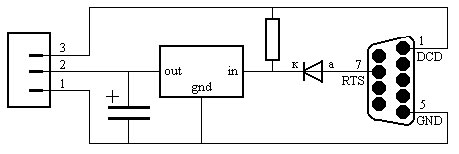
\includegraphics[width=8cm]{26_lirc_fig1}}
%\label{pic:fl1}
\caption{Схема инфракрасного приемника}
\end{figure}

\begin{figure}[ht]
\centering{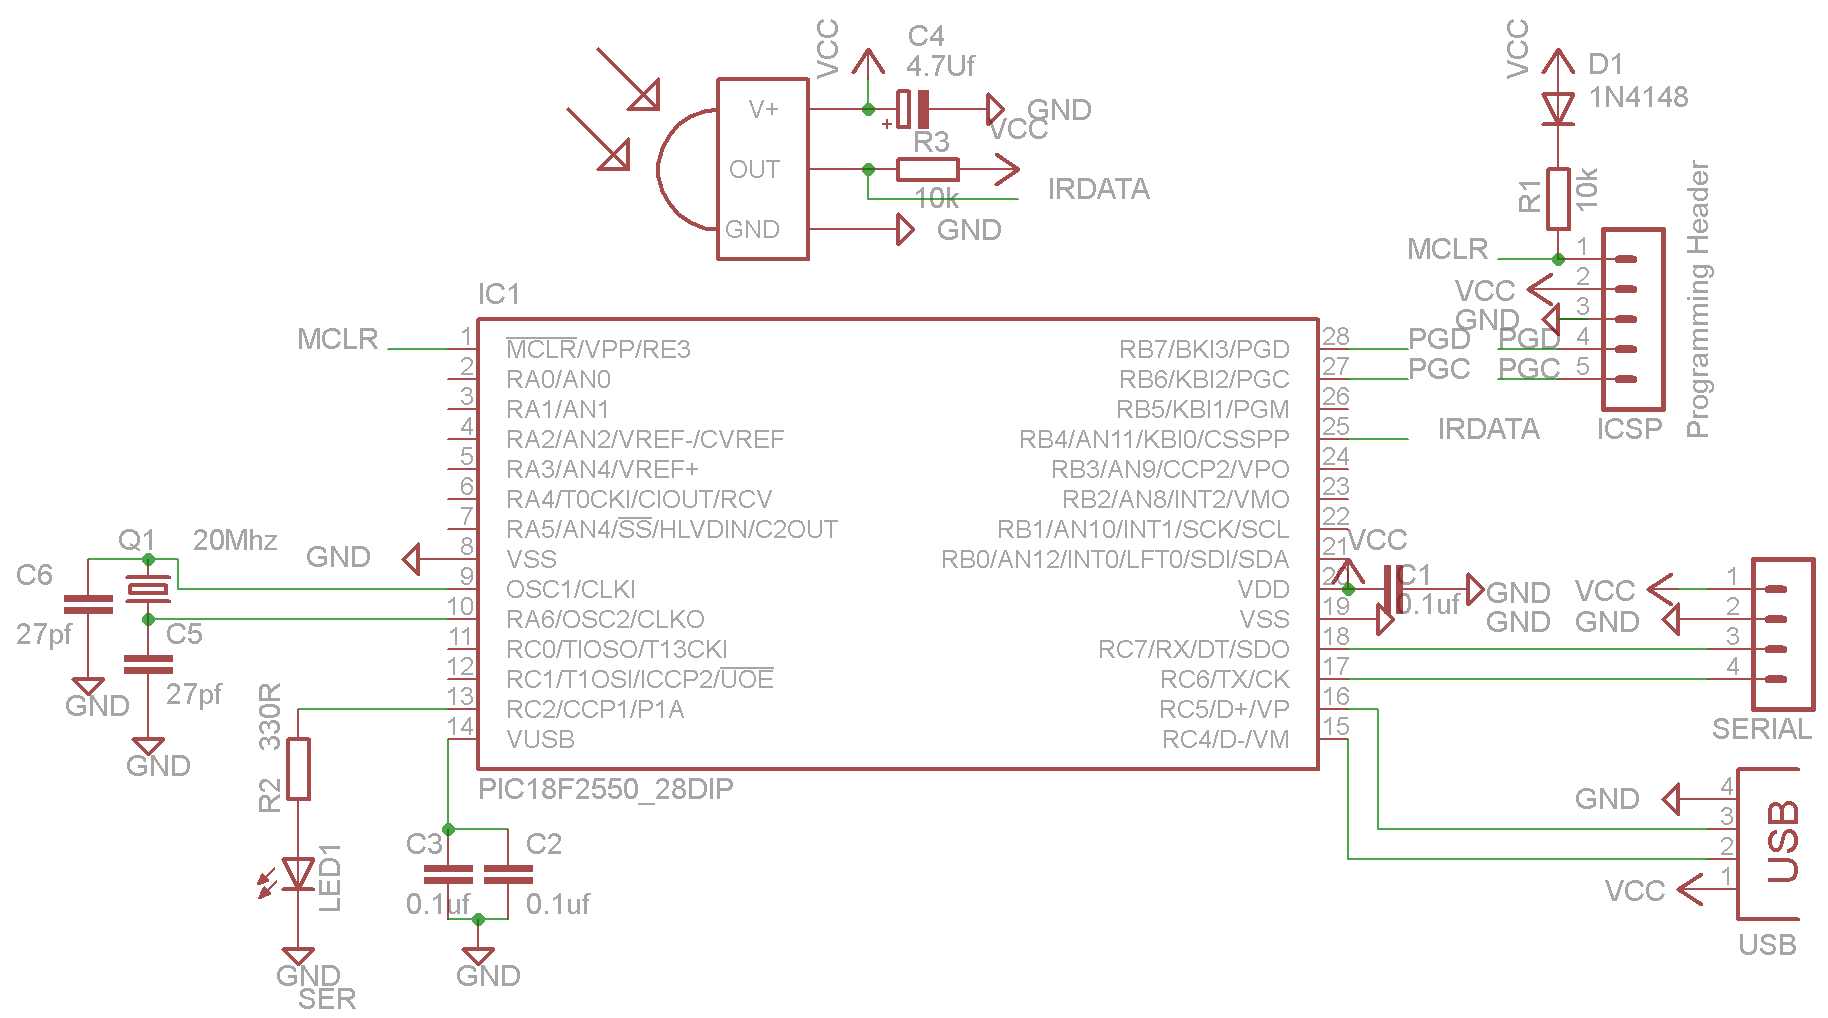
\includegraphics[width=8cm]{26_lirc_fig2}}
%\label{pic:fl1}
%\caption{Приложения по категориям}
\end{figure}

Такое решение является наиболее простым и доступным, однако, т.~к. COM-порт 
уже исчезающий вид интерфейса, более привлекательными выглядят
USB-приемники. Для его изготовления потребуется микроконтроллер.

Приемник базируется на микроконтроллере PIC18F2455, который может
работать с USB-портом и является меньшей и более дешевой версией
18F2550. Семейство 18F можно программировать при помощи универсального
PIC-программатора.

В состав пакета LIRC входят:
\begin{itemize}
	\item драйверы различных устройств (модули ядра)
	\item демон lircd, преобразующий ИК сигналы, полученные от драйвера, в стандартные сообщения, которые прикладные программы могут получить
через сокет 
\item демон lircmd, получающий сообщения от lircd и имитирующий мышь в X Windows
\item irexec "--- запуск программ по нажатию кнопки ДУ
\item irxevent "--- посылка X Windows сообщения по нажатию кнопки ДУ
\item irpty "--- псевдотерминал, запускающий программу и имитирущий нажатие клавиш клавиатуры
\end{itemize}
Кроме того, стоит упомянуть вспомогательные программы для отладки и настройки:
\begin{itemize}
	\item irrecord "--- утилита для записи сегналов пульта и создания lircd.conf
	\item irw "--- читает сообщения с сокета lircd и выдает на stdout; в качестве параметра можно указать имя сокета
	\item ircat "--- отладочная программа для конфигурационного файла ~/.lircrc; в качестве параметра указывается имя программы (точнее имя описывающей
её секции); по нажатию кнопки на пульте ДУ ircat выводит на stdout строку, привязанную к этой кнопке
\item mode2, smode2, xmode2 "--- осциллоскоп для инфракрасных сигналов
\item irsend "--- посылает команды на инфракрасные приемники (если позволяет оборудование)
\end{itemize}
В Linux существует множество приложений, направленных на централизованную работу с мультимедиа, например MythTV, Elisa,
XBMC. Однако, очевидно, что пульт может использоваться совместно с множеством других программных пакетов.

\end{document}


